\documentclass[letterpaper, 11pt]{article}
\usepackage{comment} % enables the use of multi-line comments (\ifx \fi) 
\usepackage{fullpage} % changes the margin
\usepackage{fancyhdr} % for footer
\usepackage[UKenglish]{isodate}% http://ctan.org/pkg/isodate for date format
\usepackage{wrapfig}
\usepackage[font={small,sf}]{caption}
\usepackage{float}%force tables/figs into certain placement
\usepackage{graphicx}%for figures
\graphicspath{ {./images/} }%for setting path to images uploaded to the overleaf folder
\usepackage[leftcaption]{sidecap}%for figure captions
\usepackage{subcaption}%for figures
\usepackage{hyperref}%for hyperlinks
\usepackage[font=small,labelfont=bf]{caption}%for captions
\usepackage{natbib}	%for bibliography
\usepackage{placeins}%prevent images from floating into inappropriate sections
\usepackage{tabulary}%for table at the end, to get soft wrapping
%\usepackage[capbesideposition=inside,facing=yes,capbesidesep=quad]{floatrow}
\usepackage[]{textcomp}%for degree symbol
\usepackage{titlesec}%to change appendix headers
\usepackage[titletoc,toc,title]{appendix}%to change appendix headers
\usepackage{gensymb}%for degree symbol

\usepackage{epigrafica}%changes default font to epigrafica
\usepackage[LGR,OT1]{fontenc}

%for drawing!
\usepackage{tikz}
\usetikzlibrary{shapes.geometric, arrows}


\def\labelitemi{--}

\pagestyle{fancy}
\renewcommand{\headrulewidth}{0pt}

\lhead{}
\chead{}
\rhead{}
\lfoot{Frost Entomological Museum}
\cfoot{}
\rfoot{SOP 17 --- \thepage}
\renewcommand{\footrulewidth}{0.4pt}
\title{SOP 17: Voucher specimens}
\author{Frost Entomological Museum Curator \& Interest Group}

\begin{document}
\cleanlookdateon %removed ordinal date
\maketitle
\thispagestyle{fancy}

\section*{Preamble}

The Frost Entomological Museum stands as repository for voucher specimens that represent science, surveys, and related work completed by Penn State researchers and certain affiliates. Vouchering, however, is not always straightforward. This SOP provides guidelines on how to designate vouchers for one's study and also how to get these specimens accessioned into the research collection at the Frost Entomological Museum. If you intend to deposit voucher specimens at the Frost Entomological Museum please contact Museum staff during the \textit{design phase} of your project. 

\section{Importance of vouchers}
Repeatability is a tenet of the scientific method \cite{1}. Providing others with the opportunity to verify the subject of your research---the insects and other arthropods, whose biology you investigated---is a key step in making your research repeatable. Properly prepared voucher specimens provide the means for verification and, in many cases, opportunities to build on your research \cite{2,3,4,5,6,7}. Depositing voucher specimens is as important as depositing data (e.g., DNA into NCBI's GenBank), especially for insects and other study organisms that are difficult to identify or locate in the wild. 

\section{Designating vouchers -- How many?}
The nature of your research and data collection will affect what should be vouchered, including how the arthropods were acquired, their level of taxonomic identification, the type of study the arthropods were used for, sex, life stage, or whether variants (geographic, morphological, time series, \textit{etc}.) were important aspects of the project. \textbf{A good rule of thumb is to plan for 10 voucher specimens for each type of specimen} \cite{2,5}. This approach allows you to represent the range of variability while also keeping the investment of time and resources relatively low. Exceptions to the ``10 of each type'' recommendation may include:
\begin{itemize}
\item If working with insects from a lab-reared colony, and (a) a sample of the colony has been previously vouchered and (b) there have been no changes to colony since vouchering you can probably submit fewer specimens. Contact Museum staff for a consultation.
\item If your research involved taxonomic revisions or descriptions of new species then \textit{all} of your specimens must be vouchered
\item If your research focused on broad ecological concepts, e.g., feeding guilds or all insects in a particular habitat, then contact museum staff to discuss the best vouchering strategy.
\end{itemize}

If you are unfamiliar with insect curation read our specimen preparation guide \citep{specimenPrep}. If you do not have the appropriate, archival materials, or you have questions regarding the process please contact Museum staff for assistance.

\section{Designating vouchers -- Other considerations}
\subsection{Cost}

If your research is based at Penn State University \textit{AND} you are generating a relatively small number of voucher specimens \textit{AND} you prepare the specimens and supply their associated data in an acceptable format then there is no cost. Support for materials and supplies, however, is always appreciated!

If your research will generate a large number of vouchers and/or you need assistance in making preparations and generating specimen data in an acceptable format then contact Museum staff.

\subsection{Taxonomic and other limitations}

As stated in the Collection Management Policy \citep{collectionPolicy}, there are limits to the types of specimens that can be deposited in the collection. Molluscs, vertebrates, and plants, for example, do not align with the taxonomic scope of the Frost Museum and would need to be deposited somewhere else. Physical copies of data sheets likewise should be deposited elsewhere.

\subsection{Requirements}
\begin{itemize}

\item Voucher specimens should be prepared following the Specimen Preparation Guide \cite{specimenPrep}. Voucher specimens should also be identified as such, with a separate label that includes the following:\vspace{5mm}
\tikzstyle{voucherlabel} = [rectangle, minimum width=3cm, minimum height=1cm,text centered, draw=black, fill=green!30]
\begin{tikzpicture}
\node [voucherlabel] [draw, align=left]{VOUCHER SPECIMEN \\ PhD\_ARDeans\_001};
\end{tikzpicture}

\begin{enumerate}
     \item The words "VOUCHER SPECIMEN" at the top
     \item Your name, the specimen number (unique for each specimen)
  \end{enumerate}


\item Specimen data must be submitted using the Frost Museum spreadsheet: \url{http://bit.ly/FrostVoucherData}. Additional data types (columns) can be added to the spreadsheet, but headers \textit{must be} Darwin Core terms. See \url{https://dwc.tdwg.org/terms/}

\item A statement should be included in the thesis, dissertation, or publication that indicates the vouchers were deposited at the Frost Entomological Museum at the Pennsylvania State University. The voucher number, quantity submitted, life stage and sex (if known) should be included.

\item Notify staff at the Museum when any publication based on vouchered material is accepted. You will receive a hearty congratulations(!), and specimens will be linked in the database to the article's DOI. Well done!
\end{itemize}


\clearpage
% adding bibliography here
\bibliographystyle{unsrt}
\bibliography{bib}

\end{document}


\\

\begin{figure}[ht!]
    \centering
    \begin{subfigure}[ht!]{0.43\textwidth}
        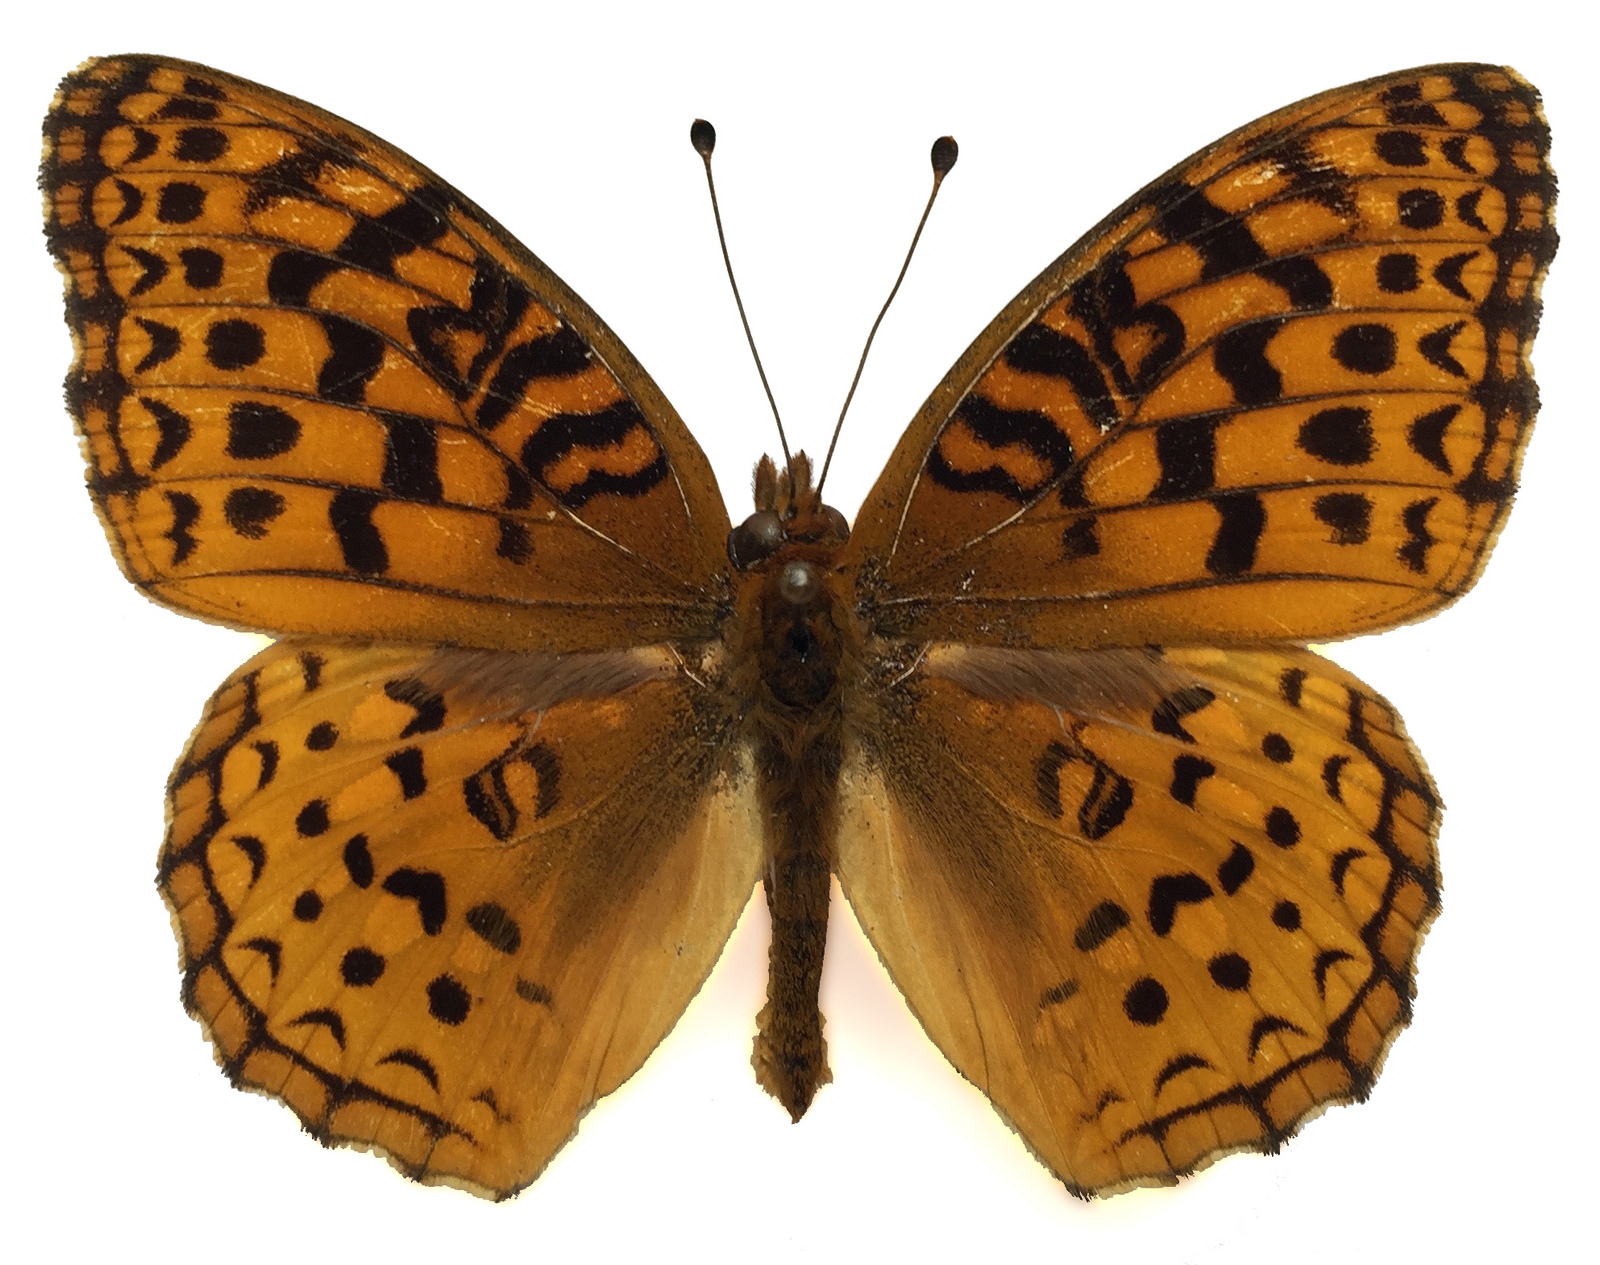
\includegraphics[width=\textwidth]{butterfly}
    \end{subfigure}
    \qquad
    \begin{subfigure}[ht!]{0.45\textwidth}
        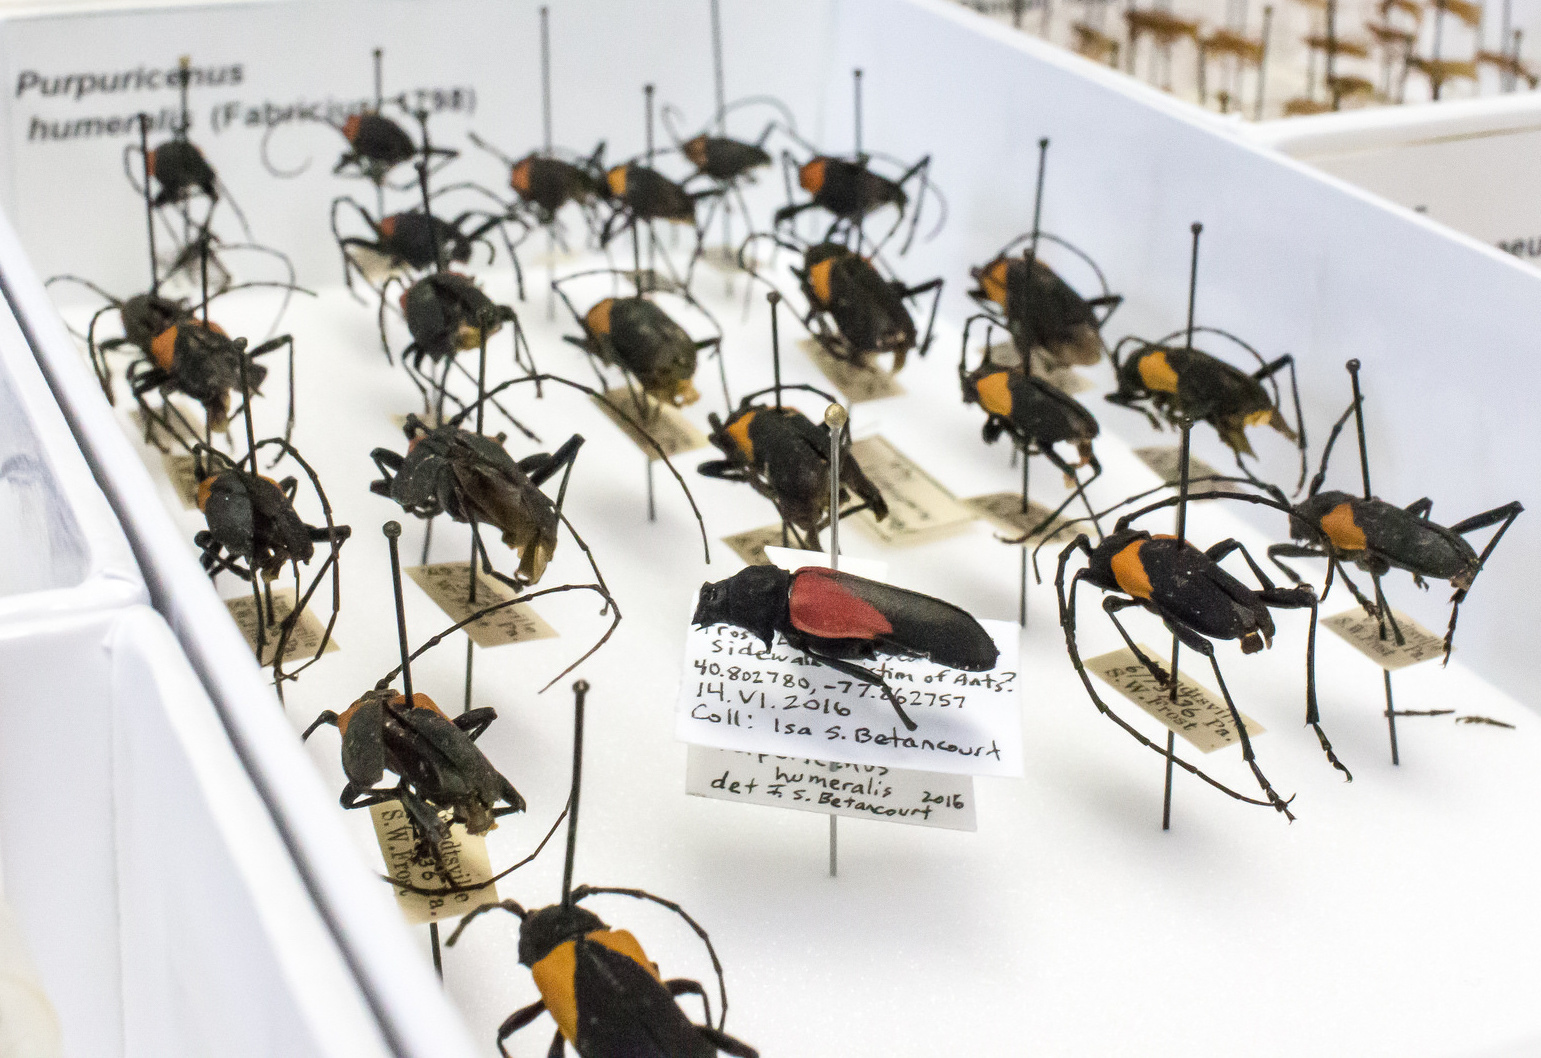
\includegraphics[width=\textwidth]{pinned}
    \end{subfigure}
    \caption{Frost Entomological Museum specimens}
\end{figure}

\begin{figure}[ht!]
	\centering
  \includegraphics[width=0.6\textwidth]{LepDamaged}
  \caption{hhhh.}
  \label{lepdestroyed}
\end{figure}
